\documentclass{article}
\usepackage{graphicx}
\usepackage{geometry}
\geometry{
 a4paper,
 total={170mm,257mm},
 left=15mm,
 top=10mm,
right=15mm,
bottom=15mm,
 }
\usepackage{enumitem}
\setlist[enumerate]{itemsep=0mm}
\setlist[itemize]{itemsep=0mm}

\begin{document}
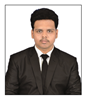
\includegraphics[scale=0.7]{smk.png}
 \textbf{\LARGE \\* \\* MAHESHKUMAR S}
\\* \large 193/16, Babu Nagar, Salem 636 001, Tamil Nadu. 
\\* \large Email ID: maheshkumar29031999@gmail.com    
\hspace{10pt}Mobile No.: +91 86950 03616  
\\*
\hrule

\textbf{\\*  \\* Career Objective}

To apply and develop my knowledge and skills in a reputed concern which will pave a way for mutual development of the concern and mine

 \textbf{\\* Education}
\\*  
\\* 
\resizebox{\textwidth}{!}{\begin{tabular}{|  c | c | c | c | c | }
 \hline
Course & Institution & Board/University & Year & Performance \\ \hline
B.E. (EEE) & Knowledge Institute of Technology, Salem. & Anna University & Pursuing & 8.42* (CGPA)\\ \hline
HSC & St.Paul’s Higher Secondary School, Salem. & State Board & 2016  & 90.33\% \\ \hline
SSLC & St.Paul’s Higher Secondary School, Salem. & State Board & 2014 & 96.80\% \\ \hline
\end{tabular}}
\\* 

\hspace{422pt} \footnotesize *upto 5\textsuperscript{th} Semester
\large
\textbf{\\* Projects}
\begin{enumerate}
\item Agribot 1.0
\item Smart Home IoT
\item Analog Line follower Robot
\item Temperature Controlled Automatic Fan Regulator
\item Car Accident Prevention System
\end{enumerate}
\begin{flushleft}
\textbf{\\* Training and Internship}
\begin{itemize}
\item Underwent One week Inplant Training on \textbf{Electrical Control Unit and Hot Rollling Mill} at JSW Pvt. Ltd. Salem, during 2018.
\item  Underwent One Week Hands-on-Training on \textbf{PCB Fabrication} conducted by Knowledge Institute of Technology, Salem as a part of Non-Formal Course, during 2017.
\item Underwent One week Inplant Training on \textbf{Electrical Maintenance, MRSS, DC and AC drives} at Steel Authority of India Limited, Salem, during 2017.
\item Underwent One week Inplant Training on\textbf{ Embedded systems} at Sans Innovations, Salem, during 2017.
\end{itemize}


\textbf{\\* Technical Skills}
\begin{itemize}
\item \textbf{Core Skills:} Robotics and Automation using Atmega 328p \& 2560 Microcontrollers, IoT using NodeMCU.
\item \textbf{Programming Skills:} C, C++ ,JAVA (Basics) 
\item \textbf{Software Tools:} MATLAB, ORCAD, Eagle, Arduino IDE, Proteus
\item \textbf{Other Skills:} Photoshop,MIT App Inventor, Cyberlink Powerdirector
\end{itemize}

\textbf{\\* Soft Skills}
\begin{enumerate}
\item Leadership
\item Time Management
\item Team Work
\item Logical reasoning
\item Work Ethic
\end{enumerate}

\textbf{\\* Extra Curricular Activities}
\begin{itemize}
\item \textbf{Designig Posters and Brouchers} for Symposium for the academic year 2017-18 and 2018-19 using Photoshop.
\item \textbf{Singing} - Won prizes in College Culturals in the year 2017 and 2018 .
\item Participated in  \textbf{CYBER WARRIORS} program conducted by Salem City Police - 2018.
\item Participated in \textbf{Dengue Awareness program} to create awareness among rural people - 2018.
\item Participated as a Volunteer for \textbf{Blood Donation Camp} conducted by Lions Club, Salem - 2017.
\item Participated in \textbf{ICT Academy Youth Leadership Summit 2016} organized by ICT Academy held at Codissia Trade Fair Complex, Coimbatore – 2016.
\end{itemize}

\textbf{\\* Roles and Responsibiities}
\begin{itemize}
\item Active Member of \textbf{IIC-MHRD}, 2018-19.
\item Active Member of \textbf{Indian Society for Technical Education} (ISTE), 2018-19.
\item \textbf{Joint Secretary} of AMBERZ’ Electrical Engineer's Association, Knowledge Institute of Technology, Salem  for academic year 2018-19.
\item \textbf{Placement Ambassador} of EEE at Knowledge Institute of Technology, Salem during 2017-18 and 2018-19.
\item Member of \textbf{Youth Red Cross} (YRC) club during 2016-17.
\end{itemize}

 \textbf{\\* Co-Curricular Activities}
\\*
\begin{enumerate}
\item \textbf{Contests and Presentations}
\begin{itemize}
\item Won \textbf{Judges Choice Award} for the project titled \textbf{Agribot 1.0} in National Finals of \textbf{e-Yantra Ideas Competition 2019}, conducted by IIT Bombay.
\item Won \textbf{Third Prize} in paper presentation titled on \textbf{Smart Home IoT} during EDISON 2018, A National level Technical symposium at Sona College of Technology, Salem - 2018.
\item Won \textbf{Third Prize} in Paper Presentation titled on \textbf{Temperature Controlled Automatic Fan Regulator} during SCIENTEL 2018 – A National level Technical symposium at Government College of Engineering, Salem - 2018.
\item Won \textbf{Second Prize} in Make a Product Expo titled on Temperature Controlled Automatic Fan Regulator conducted by AMBERZ’ association, Knowledge Institute of Technology, Salem - 2018.
\item Won \textbf{First Prize} for the paper on \textbf{Language is Power} during COLLOQIA 2016 – A National level Technical Symposium at M Kumarasamy College of Engineering, Karur.
\item Won \textbf{Second Prize} for the paper on \textbf{Hospital Management and Emergency Mobility System } during 2016,  A National level Technical Symposium at Dhirajlal Gandhi College of Technology, Salem. 
\item Received \textbf{ Best Co-curricular Activity} award at Valedictory of AMBER'Z Association 2018-19, conducted by Knowledge Institute of Technology Salem.
\item Received \textbf{ Best Co-curricular Activity} award at Annual day Awards 2016-17, conducted by Knowledge Institute of Technology Salem.
\end{itemize}

\item \textbf{Workshops and seminars}
\begin{itemize}
\item \textbf{PLC and SCADA} Workshop at Karpagam College of Engineering, Coimbatore.
\item \textbf{Robotics using Arduino} Workshop by Master Technologies, Salem.
\item\textbf{IOT Home Guard} using Arduino Workshop by Top Engineers, IIT Madras.
\item\textbf{Recent Technologies in Autonomous and Hybrid Vehicles} Seminar by IEEE at Knowledge Institute of Technology, Salem.
\item \textbf{Solar PV} Seminar by Indian Society for Technical Engineering at Knowledge Institute of Technology, Salem. 

\end{itemize}
\end{enumerate}

\textbf{\\*  Certifications}
\begin{itemize}
\item Received Completion certificate for \textbf{C and C++}, by \textbf{Spoken Tutoria}l Project, IIT Bombay, funded by National Mission on Education through ICT, MHRD, Govt. of India.
\item Got \textbf{Winner Certificate} for an outstanding performance on achieving First Place in the \textbf{Basic Electrical and Electronics} - an online contest by TI University Program.
\item Received \textbf{Certificate of Merit} in recognition of excellent performance in the {Electronic Devices and Circuits, Digital Signal Processing, Linear Integrated Circuits} - online contests by \textbf{TI University Program}.
\item Received Certification for Completion of \textbf{AUTOCAD} conducted by State Project Co-ordination Unit, established under \textbf{Canada India Institutional Co-operation Project}.
\end{itemize}
\end{flushleft}

\textbf{\\* Personal Information} 
\\* 
\\*
\hspace*{8pt}
\begin{tabular}{ l l l }
Father's Name & : & A.N.Santharam \\ 
Mother's Name & : & J.Bhuvana\\ 
Sex & : & Male \\ 
Date of Birth & : & 29.03.1999 \\ 
Nationality & : & Indian \\
\end{tabular}
\\* 

\textbf{\\* Reference}
\begin{itemize}
\item
\begin{description}
\item  Dr.C.Muniraj, M.E., Ph.D.,
\item  Professor \& Head, Department Electrical and Electronics Engineering.
\item  Knowledge Institute of Technology, Salem, Tamil Nadu.
\item  hod.eee@kiot.ac.in
\\*
\end{description}

\item
\begin{description}
\item  Mr.L.Manivannan, M.E.,
\item  Assistant Professor,Department of  Electrical and Electronics Engineering.
\item  Knowledge Institute of Technology, Salem, Tamil Nadu.
\item  lmeee@kiot.ac.in
\end{description}
\end{itemize}

\end{document}